\documentclass{beamer}

\usepackage{lmodern}
\usepackage[utf8]{inputenc}
\usepackage{hyperref}
\usepackage{tabularx}
\usepackage{siunitx}
\sisetup{output-exponent-marker=\ensuremath{\mathrm{e}}}

\usetheme{Madrid}
\usecolortheme{default}

%------------------------------------------------------------
\title[About Beamer]
{About the Beamer class in presentation making}

\subtitle{A short story}

\author[Claudio, Jos\'e]
{Claudio Scheer\inst{1} \and Jos\'e Fernando Possebon\inst{1}}

\institute[PUCRS]
{
  \inst{1}%
  Pontifical Catholic University of Rio Grande do Sul - PUCRS\\
  \{claudio.scheer, jose.possebon\}@edu.pucrs.br
}

\date[Deep Learning 2020]
{Deep Learning, June 2020}


\AtBeginSection[]
{
  \begin{frame}
    \frametitle{Table of Contents}
    \tableofcontents[currentsection]
  \end{frame}
}
%------------------------------------------------------------


\begin{document}

\frame{\titlepage}


%---------------------------------------------------------
\begin{frame}
  \frametitle{Table of Contents}
  \tableofcontents
\end{frame}
%---------------------------------------------------------


%---------------------------------------------------------
\section{Proposal}

\begin{frame}
  \frametitle{Proposal}

  % \begin{itemize}
  %   \item<1-> Text visible on slide 1
  %   \item<2-> Text visible on slide 2
  %   \item<3> Text visible on slides 3
  %   \item<4-> Text visible on slide 4
  % \end{itemize}
\end{frame}

% \begin{frame}
%   In this slide \pause

%   the text will be partially visible \pause

%   And finally everything will be there
% \end{frame}
%---------------------------------------------------------


%---------------------------------------------------------
\section{Dataset}

\begin{frame}
  \frametitle{The Enron Email Dataset}

  {\scriptsize
    no, i dont mind.       : - )
    \bigbreak
    -----Original Message-----
    \bigbreak
    Hi how are you doing?  I have a meeting from 4 to 5, do you mind waiting for me?  Thanks.
    
    John
    \bigbreak
    -----Original Message-----
    \bigbreak
    hello
  }
\end{frame}

\begin{frame}
  \frametitle{The Enron Email Dataset}

  \begin{itemize}
    \item \href{https://www.kaggle.com/claudioscheer/extract-reply-emails}{https://www.kaggle.com/claudioscheer/extract-reply-emails};
    \item Get only emails with less than 256 characters;
  \end{itemize}

  \bigbreak
  \bigbreak
  \bigbreak

  Final dataset: \num{40062} input-target pairs.
  \\
  Train dataset: \num{10002} input-target pairs.
\end{frame}

\begin{frame}
  \frametitle{Samples}

  \begin{table}
    \centering
    \begin{tabularx}{\textwidth}{|X|X|}
      \hline
      \textbf{Input}                                                            & \textbf{Target}                                                                       \\
      \hline
      I thought this one was canceled. So I declined to get it off my calendar. & You're right.                                                                         \\
      \hline
      Rex - thanks for the quick response...please note the revised letters below.
      Previous email had a clerical error                                       & Who will sign theses?                                                                 \\
      \hline
      Where can I get info on safety statistics for the pipes?                  & Ralph, please get with Rod and provide what ever he needs in the way of Safety Stats. \\
      \hline
    \end{tabularx}
  \end{table}
\end{frame}
%---------------------------------------------------------


%---------------------------------------------------------
\section{BERT}

\begin{frame}
  \frametitle{BERT architecture}
\end{frame}

\begin{frame}
  \frametitle{Hugging Face}

  \begin{itemize}
    \item BERT base was used;
          \begin{itemize}
            \item 12 layers;
          \end{itemize}
    \item Hugging Face and PyTorch was used;
  \end{itemize}
\end{frame}

\begin{frame}
  \frametitle{Learning Rate Schedule}

  \begin{itemize}
    \item Warm-up steps: \num{10000};
    \item Learning rate: \num{1e-4};
  \end{itemize}

  \bigbreak
  \bigbreak

  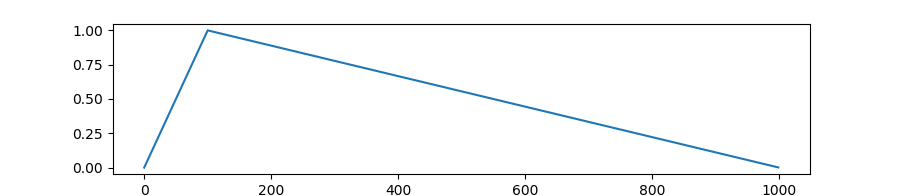
\includegraphics[width=\textwidth]{../images/warmup_linear_schedule.png}
\end{frame}

\begin{frame}
  \frametitle{Optimizer and hyperparameters}

  \begin{itemize}
    \item Adam;
          \begin{itemize}
            \item Adam epsilon: \num{1e-4};
          \end{itemize}
    \item Batch size: \num{8};
    \item Training epochs: \num{32};
    \item Beam search hypothesis: \num{3};
  \end{itemize}
\end{frame}
%---------------------------------------------------------


%---------------------------------------------------------
\section{Results}

\begin{frame}
  \frametitle{Generated replies}

  \begin{table}
    \centering
    \begin{tabularx}{\textwidth}{|X|X|c|}
      \hline
      \textbf{Email}                      & \textbf{Reply}                                                                              & \textbf{AI?} \\
      \hline
      Shall we have the meeting tomorrow? & meeting is postponed because the 3 : 00 p. m. meeting today. meeting is canceled for today. & \num{30}{\%} \\
      \hline
      hi                                  & Hi how are you?                                                                             & \num{10}{\%} \\
      \hline
      you look so handsome today          & why thank you, you do as well                                                               & \num{30}{\%} \\
      \hline
    \end{tabularx}
  \end{table}
\end{frame}
%---------------------------------------------------------

\end{document}